\section{Proofs}
\label{app:proofs}
Notation as in Section~\ref{sec:theory}; $Q=\Lambda_S^\top\Psi_S^{-1}\Lambda_S\succeq0$ has rank at most $k=|S|$ and $P_S=(I+Q)^{-1}$.

\paragraph{Proposition~\ref{prop:decomp}.}
Given $x_S$, $z\mid x_S\sim\mathcal N(m_S,P_S)$ where $m_S$ is linear in $x_S$ and $P_S$ does not depend on $x_S$.
For $j\in T$ the Bayes predictor is $\hat x_j=\mu_j+\lambda_j^\top m_S$, and $x_j-\hat x_j=\lambda_j^\top(z-m_S)+\varepsilon_j$ with $\varepsilon_j$ independent of $z-m_S$, so $\mathbb{E}(x_j-\hat x_j)^2=\lambda_j^\top P_S\lambda_j+\psi_j$; summing over $T$ gives $\sum_{T}\psi_j+\mathrm{tr}(W_TP_S)$.
For an adaptive policy the set $S_\tau$ after $\tau$ steps is a function of earlier scores; its final error is $\mathbb{E}[\mathrm{err}(S_k)]$ with $\mathrm{err}(S)$ the above, which depends on $S$ only, so $\mathbb{E}[\mathrm{err}(S_k)]\ge\min_{|S|=k}\mathrm{err}(S)$. (For targets that are the complement of $S$ the same argument applies, with $T=T(S)$.) \qed

\paragraph{Proposition~\ref{prop:floor}.}
$P_S$ and $Q$ commute and share eigenvectors. Let $\Pi$ be the orthogonal projector on $\mathrm{range}(Q)$, $\mathrm{rank}\,\Pi\le k$. On $\mathrm{range}(Q)^\perp$, $P_S$ is the identity; on $\mathrm{range}(Q)$ it is positive semidefinite. Hence $P_S\succeq I-\Pi$ and $\mathrm{tr}(W_TP_S)\ge\mathrm{tr}(W_T)-\mathrm{tr}(W_T\Pi)$.
By Ky Fan's inequality $\mathrm{tr}(W_T\Pi)\le\sum_{i\le k}\lambda_i(W_T)$, and $\mathrm{tr}\,W_T=\sum_i\lambda_i(W_T)$, so $\mathrm{tr}(W_TP_S)\ge\sum_{i>k}\lambda_i(W_T)$. For the complement $T=T(S)$, $W_T=\Lambda^\top\Lambda-\Lambda_S^\top\Lambda_S$ is a perturbation by a PSD matrix of rank $\le k$, so $\lambda_i(W_T)\ge\lambda_{i+k}(\Lambda^\top\Lambda)$ (Weyl). \qed

\paragraph{Block case and water-filling.}
Let each benchmark load on exactly one factor, $\lambda_j=\ell_j e_{i(j)}$, and let $S$ contain $k_i$ benchmarks of factor $i$ with signal-to-noise $\rho_{ij}=\ell_j^2/\psi_j$. Then $Q$ is diagonal with entries $q_i=\sum_{j\in S,i(j)=i}\rho_{ij}$, $P_S=\mathrm{diag}(1/(1+q_i))$ and $\mathrm{tr}(W_TP_S)=\sum_iW_{ii}/(1+q_i)$. With equal $\rho_{ij}=\rho_i$, $q_i=k_i\rho_i$. Minimising over integers $k_i$ with $\sum k_i=k$ is a separable convex problem whose continuous relaxation is solved by reverse water-filling, $1+k_i\rho_i=\sqrt{W_{ii}\rho_i/\nu}$ for a multiplier $\nu$, truncated at $k_i=0$. For $r$ balanced factors ($W_{ii}=W$, $\rho_i=\rho$) the error on the latent part equals $W r/(1+k\rho/r)$, and the latent error reaches a fraction $\delta$ of its initial value $Wr$ at $k=r(1/\delta-1)/\rho$. \qed

\paragraph{Greedy guarantee.}
\label{app:greedy}
Write $f_W(S)=\mathrm{tr}\,W(I-P_S)=\sum_tw_t\mathrm{Var}(s_t)R^2_t(S)$ for $W=\sum_tw_tu_tu_t^\top$, $s_t=u_t^\top z$ and $R^2_t(S)$ the squared multiple correlation of $s_t$ with $x_S$. This is a non-negative combination of variance-explained functions whose submodularity ratio is bounded below by the smallest eigenvalue of the correlation matrix of the observed scores restricted to subsets of bounded size \citep{das2011submodular}; the ratio of a non-negative combination is at least the smallest ratio of its terms, so greedy maximisation of $f_W$ is within $1-e^{-\gamma}$ of the optimum for a fixed $W$. The complement-error criterion is not of this form, because $T$ moves with $S$.

\paragraph{Greedy against the best set found.}
For the fitted factor model of each fold of the first repetition, $f_W$ of the greedy set is compared with that of the best set found for the all-latent weight: by exhaustive search for $k\le4$ ($k\le3$ on A1) and by swap local search started from the greedy set for larger $k$, so for $k\ge4$ the comparison set is the best found, not a certified optimum. The median ratio is $0.948$ ($k=2$), $0.986$, $0.988$, $0.992$ ($k=8$) and $0.997$ ($k=12$) on A1, with minimum $0.947$ over folds and $k$, and $0.975$, $0.983$, $0.998$, $0.999$, $1.000$ on A2 with minimum $0.965$. The complement error of the greedy set is at most $13\%$ above that of the best set found. The estimated submodularity ratio is $\gamma\approx0.010$--$0.024$ for $k\ge2$ ($0.98$ at $k=1$), so $1-e^{-\gamma}\approx0.01$--$0.02$. The sets chosen differ between folds on A1 (mean pairwise Jaccard $0.12$--$0.16$; A2 $0.30$--$0.61$) while their objective values are near-optimal, so the optimum is flat there and individual selected benchmarks should not be interpreted.

\section{Data}
\label{app:data}
\begin{table}[h]
\centering\scriptsize\setlength{\tabcolsep}{3pt}
\begin{tabular}{@{}lrrrrrrrl@{}}
\toprule
Matrix & $M$ & $N$ & density & top-eig. share & part. ratio & FA rank & $h$ & version \\
\midrule
MTEB-A1 & 103 & 202 & 1.00 & 0.57 & 2.9 & 8 & 0.85 & 6dabbcc68c28 \\
MTEB-A2 & 126 & 30 & 1.00 & 0.67 & 2.1 & 4 & 0.84 & 6dabbcc68c28 \\
MTEB-B & 507 & 598 & 0.22 & 0.28 & 9.5 & 2 & 0.75 & 6dabbcc68c28 \\
OLLB v2 (40 subtasks) & 4508 & 40 & 1.00 & 0.61 & 2.6 & 8 & 0.81 & aa81ecc38fdc \\
OLLB v2 (6 benchmarks) & 4576 & 6 & 1.00 & 0.73 & 1.8 & 3 & 0.79 & 9c09a7cae433 \\
HELM MMLU & 79 & 57 & 1.00 & 0.80 & 1.6 & 3 & 0.89 & v1.13.0 \\
HELM Lite & 91 & 10 & 1.00 & 0.63 & 2.3 & 2 & 0.79 & v1.13.0 \\
LiveBench & 195 & 7 & 0.77 & 0.68 & 2.0 & 3 & 0.88 & 9704e5da7bfb \\
\bottomrule
\end{tabular}

\caption{Matrices. $M$ models, $N$ benchmarks, share of observed cells, share of variance in the top eigenvalue of the correlation matrix, participation ratio of its eigenvalues, median factor-analysis rank over the fold fits (chosen by held-out likelihood), median latent share $h$ of variance, and the data version. Sources and licences: Table~\ref{tab:sources}.}
\label{tab:t1}
\end{table}
The matrices differ in the structure the method relies on (Table~\ref{tab:t1}): the embedding blocks A1 and A2 are complete and have one dominant direction (top eigenvalue share $0.57$ and $0.67$) with a participation ratio of $2$--$3$ and a factor-analysis rank of $8$ and $4$; the sparse matrix B has a weaker leading direction ($0.28$) and a participation ratio of $9.5$ but a fitted rank of only $2$ (with $22\%$ of its cells observed); the generative-LLM matrices have fitted ranks of $2$ to $3$, and $8$ on the 40 Open LLM Leaderboard subtasks.

\begin{table}[h]
\centering\scriptsize\setlength{\tabcolsep}{3pt}
\begin{tabular}{@{}lp{0.33\textwidth}p{0.13\textwidth}p{0.22\textwidth}@{}}
\toprule
Matrix & source & version & licence \\
\midrule
MTEB-A1 & MTEB results repo (embeddings-benchmark/results), peeled complete block & git 6dabbcc68c28 & CC0-1.0 (GitHub repository licence, checked via API 2026-11-18) \\
MTEB-A2 & MTEB results repo, 30 most-covered tasks & git 6dabbcc68c28 & as A1 \\
MTEB-B & MTEB results repo, sparse block & git 6dabbcc68c28 & as A1 \\
OLLB v2 (40 subtasks) & Open LLM Leaderboard v2 per-subtask results (HF open-llm-leaderboard/results) & commit aa81ecc38fdc & none stated on dataset \\
OLLB v2 (6 benchmarks) & Open LLM Leaderboard v2 contents (HF) & commit 9c09a7cae433 & none stated on dataset card \\
HELM MMLU & HELM MMLU 57 subjects (crfm-helm-public) & v1.13.0 & none stated in bucket; HELM code Apache-2.0 \\
HELM Lite & HELM Lite (crfm-helm-public) & v1.13.0 & none stated in bucket; HELM code Apache-2.0 \\
LiveBench & LiveBench model\_judgment (HF), 7-task snapshot & commit 9704e5da7bfb & none stated on dataset card \\
\bottomrule
\end{tabular}

\caption{Sources, versions and licences of the matrices of Table~\ref{tab:t1}. A source whose licence is stated nowhere on the dataset is marked ``none stated''; only scores are used.}
\label{tab:sources}
\end{table}

\section{Leakage in the protocol}
\label{app:protocol}
\begin{table}[h]
\centering\scriptsize\setlength{\tabcolsep}{4pt}
\begin{tabular}{@{}llrrr@{}}
\toprule
Matrix & $k$ & RMSE, history only & RMSE, test models in history & $\Delta$MSE [95\% CI] \\
\midrule
A1 & 3 & 0.595 & 0.535 & $-$0.068 [$-$0.096, $-$0.045] \\
A1 & 8 & 0.549 & 0.450 & $-$0.099 [$-$0.128, $-$0.073] \\
A1 & 20 & 0.492 & 0.381 & $-$0.097 [$-$0.122, $-$0.075] \\
A2 & 3 & 0.564 & 0.506 & $-$0.062 [$-$0.103, $-$0.031] \\
A2 & 8 & 0.430 & 0.385 & $-$0.036 [$-$0.053, $-$0.023] \\
A2 & 20 & 0.333 & 0.266 & $-$0.040 [$-$0.074, $-$0.019] \\
\bottomrule
\end{tabular}
\caption{Error when the standardisation, factor model and selection use the test models as well as the history, against the protocol of Section~\ref{sec:setting}; complement-error greedy$^\dagger$, factor inference; $\Delta$MSE is the former minus the latter, with 95\% intervals over $103$ (A1) and $126$ (A2) held-out models, five repetitions of 5-fold splits. The intervals exclude zero for factor, Gaussian-conditional and ridge inference and for the other selectors as well. The history-mean predictor moves too (A1: RMSE $1.03$ to $0.995$), so part of the apparent gain is the standardisation seeing the test models.}
\end{table}

\section{All primary comparisons}
\label{app:t2full}
\begin{table}[h]
\centering\scriptsize\setlength{\tabcolsep}{3pt}
\begin{tabular}{@{}lrrr@{}}
\toprule
Comparison & $k=3$ & $k=8$ & $k=20$ \\
\midrule
\multicolumn{4}{@{}l}{\textit{MTEB-A1}} \\
P1 A-optimal vs random & \textbf{$-$28 [$-$33,$-$22]} & \textbf{$-$15 [$-$19,$-$10]} & \textbf{$-$3 [$-$5,$-$2]} \\
P3 A-optimal vs cluster & $+$3 [$-$1,$+$10] & $-$2 [$-$5,$+$1] & \textbf{$+$3 [$+$2,$+$5]} \\
P3 A-optimal vs pivqr & \textbf{$-$42 [$-$48,$-$35]} & \textbf{$-$40 [$-$47,$-$34]} & \textbf{$-$17 [$-$22,$-$12]} \\
P3 A-optimal vs leverage & \textbf{$-$61 [$-$74,$-$48]} & \textbf{$-$53 [$-$63,$-$43]} & \textbf{$-$23 [$-$31,$-$17]} \\
P3 A-optimal vs central & \textbf{$-$25 [$-$33,$-$19]} & \textbf{$-$29 [$-$41,$-$20]} & \textbf{$-$18 [$-$25,$-$13]} \\
P5 FA vs ridge (A-optimal) & 0 [$-$2,$+$2] & $+$2 [$-$1,$+$7] & \textbf{$+$7 [$+$5,$+$9]} \\
P5 FA vs kNN (A-optimal) & $+$9 [$+$2,$+$15] & $+$6 [$-$1,$+$13] & 0 [$-$6,$+$5] \\
P5 FA vs softImpute (A-optimal) & \textbf{$-$21 [$-$28,$-$14]} & \textbf{$-$11 [$-$17,$-$5]} & $+$2 [$-$1,$+$4] \\
P7 complement-error greedy vs A-optimal\,$\dagger$ & 0 & 0 [0,$+$1] & \textbf{$-$12 [$-$16,$-$9]} \\
P7 complement-error greedy vs random\,$\dagger$ & \textbf{$-$28 [$-$33,$-$22]} & \textbf{$-$15 [$-$18,$-$10]} & \textbf{$-$15 [$-$19,$-$12]} \\
P8 greedy-Gauss+gcov vs A-optimal+fa\,$\dagger$ & 0 [$-$2,$+$3] & $-$2 [$-$5,$+$1] & \textbf{$-$20 [$-$24,$-$17]} \\
P8 greedy-Gauss+gcov vs random+gcov\,$\dagger$ & \textbf{$-$28 [$-$33,$-$23]} & \textbf{$-$14 [$-$16,$-$11]} & \textbf{$-$15 [$-$18,$-$12]} \\
\midrule
\multicolumn{4}{@{}l}{\textit{MTEB-A2}} \\
P1 A-optimal vs random & \textbf{$-$20 [$-$25,$-$15]} & $-$3 [$-$9,$+$4] & \textbf{$+$52 [$+$36,$+$72]} \\
P3 A-optimal vs cluster & $+$2 [$-$4,$+$8] & \textbf{$+$16 [$+$8,$+$25]} & \textbf{$+$90 [$+$65,$+$122]} \\
P3 A-optimal vs pivqr & \textbf{$-$23 [$-$34,$-$9]} & $+$17 [$+$2,$+$35] & \textbf{$+$249 [$+$188,$+$324]} \\
P3 A-optimal vs leverage & \textbf{$-$45 [$-$57,$-$33]} & $-$6 [$-$17,$+$6] & \textbf{$+$83 [$+$57,$+$117]} \\
P3 A-optimal vs central & \textbf{$-$6 [$-$9,$-$2]} & \textbf{$-$21 [$-$38,$-$9]} & \textbf{$-$19 [$-$31,$-$9]} \\
P5 FA vs ridge (A-optimal) & 0 [$-$1,$+$1] & \textbf{$+$5 [$+$2,$+$9]} & \textbf{$+$20 [$+$12,$+$31]} \\
P5 FA vs kNN (A-optimal) & \textbf{$+$25 [$+$13,$+$40]} & $+$6 [0,$+$12] & $+$10 [$+$2,$+$18] \\
P5 FA vs softImpute (A-optimal) & \textbf{$-$13 [$-$18,$-$9]} & \textbf{$-$7 [$-$11,$-$2]} & \textbf{$+$11 [$+$7,$+$16]} \\
P7 complement-error greedy vs A-optimal\,$\dagger$ & 0 [$-$3,$+$3] & \textbf{$-$30 [$-$45,$-$17]} & \textbf{$-$67 [$-$88,$-$50]} \\
P7 complement-error greedy vs random\,$\dagger$ & \textbf{$-$20 [$-$24,$-$16]} & \textbf{$-$32 [$-$45,$-$21]} & \textbf{$-$50 [$-$65,$-$37]} \\
P8 greedy-Gauss+gcov vs A-optimal+fa\,$\dagger$ & 0 [$-$6,$+$5] & \textbf{$-$28 [$-$45,$-$16]} & \textbf{$-$72 [$-$94,$-$53]} \\
P8 greedy-Gauss+gcov vs random+gcov\,$\dagger$ & \textbf{$-$20 [$-$27,$-$15]} & \textbf{$-$27 [$-$42,$-$16]} & \textbf{$-$47 [$-$62,$-$34]} \\
\midrule
\multicolumn{4}{@{}l}{\textit{MTEB-B (three repetitions)}} \\
P1 A-optimal vs random & \textbf{$-$22 [$-$25,$-$18]} & $-$2 [$-$4,$+$1] & \textbf{$+$14 [$+$9,$+$22]} \\
P2, P3 A-optimal vs most-covered & \textbf{$-$28 [$-$36,$-$21]} & \textbf{$-$18 [$-$24,$-$13]} & 0 [$-$5,$+$6] \\
P3 A-optimal vs pivqr & $-$4 [$-$7,$-$1] & $+$10 [$-$1,$+$24] & \textbf{$+$35 [$+$17,$+$58]} \\
P3 A-optimal vs central & \textbf{$-$22 [$-$27,$-$17]} & \textbf{$-$13 [$-$15,$-$11]} & \textbf{$-$8 [$-$11,$-$4]} \\
P5 FA vs ridge (A-optimal) & \textbf{$+$1 [$+$1,$+$2]} & \textbf{$+$7 [$+$6,$+$8]} & \textbf{$+$21 [$+$17,$+$27]} \\
P5 FA vs kNN (A-optimal) & \textbf{$+$10 [$+$7,$+$13]} & \textbf{$+$14 [$+$10,$+$17]} & \textbf{$+$19 [$+$15,$+$23]} \\
P5 FA vs softImpute (A-optimal) & \textbf{$-$22 [$-$26,$-$18]} & \textbf{$-$7 [$-$10,$-$4]} & \textbf{$+$10 [$+$4,$+$15]} \\
P7 complement-error greedy vs A-optimal\,$\dagger$ & 0 [0,0] & \textbf{$-$2 [$-$2,$-$1]} & \textbf{$-$26 [$-$44,$-$12]} \\
P7 complement-error greedy vs random\,$\dagger$ & \textbf{$-$22 [$-$25,$-$18]} & $-$3 [$-$6,$-$1] & \textbf{$-$15 [$-$29,$-$5]} \\
P8 greedy-Gauss+gcov vs A-optimal+fa\,$\dagger$ & \textbf{$+$28 [$+$22,$+$36]} & $+$3 [$-$2,$+$9] & \textbf{$-$29 [$-$48,$-$16]} \\
P8 greedy-Gauss+gcov vs random+gcov\,$\dagger$ & \textbf{$-$9 [$-$14,$-$5]} & $-$1 [$-$3,$+$1] & \textbf{$-$12 [$-$25,$-$4]} \\
\bottomrule
\end{tabular}

\caption{The comparisons of the primary family on each MTEB matrix (twelve on A1 and A2, of which Table~\ref{tab:t2} shows eight; B has three repetitions of five folds, no cluster or leverage selection, and a Holm family of 33 tests): relative change in held-out MSE (\%), first named minus second; conventions as in Table~\ref{tab:t2}.}
\label{tab:t2full}
\end{table}

\begin{table}[h]
\centering\scriptsize\setlength{\tabcolsep}{3pt}
\begin{tabular}{@{}lrrr@{}}
\toprule
Comparison & \multicolumn{3}{c}{change in MSE (\%)} \\
\midrule
\multicolumn{4}{@{}l}{\textit{Open LLM Leaderboard, 40 subtasks}, $k=3, 8, 20$; Holm family of 30} \\
P1 A-optimal vs random & \textbf{$-$23 [$-$24,$-$21]} & \textbf{$-$12 [$-$13,$-$11]} & $+$1 [$-$1,$+$3] \\
P3 A-optimal vs pivqr & \textbf{$-$34 [$-$37,$-$32]} & \textbf{$-$13 [$-$16,$-$11]} & \textbf{$+$99 [$+$94,$+$104]} \\
P5 FA vs ridge & \textbf{$-$1 [$-$1,$-$1]} & 0 [$-$1,0] & \textbf{$+$5 [$+$4,$+$6]} \\
P7 complement-error greedy vs A-optimal\,$\dagger$ & \textbf{$-$2 [$-$4,$-$1]} & \textbf{$-$15 [$-$16,$-$13]} & \textbf{$-$50 [$-$52,$-$47]} \\
P7 complement-error greedy vs random\,$\dagger$ & \textbf{$-$25 [$-$26,$-$23]} & \textbf{$-$25 [$-$26,$-$24]} & \textbf{$-$49 [$-$52,$-$47]} \\
\midrule
\multicolumn{4}{@{}l}{\textit{Open LLM Leaderboard, 6 benchmarks}, $k=2, 3$; Holm family of 22} \\
P1 A-optimal vs random & \textbf{$-$3 [$-$4,$-$2]} & \textbf{$+$7 [$+$5,$+$9]} & -- \\
P3 A-optimal vs pivqr & $+$1 [$-$1,$+$2] & \textbf{$+$27 [$+$22,$+$31]} & -- \\
P5 FA vs ridge & \textbf{$-$4 [$-$4,$-$3]} & \textbf{$-$4 [$-$4,$-$3]} & -- \\
P5 FA vs kNN & \textbf{$+$10 [$+$8,$+$12]} & \textbf{$+$29 [$+$25,$+$32]} & -- \\
P5 FA vs softImpute & \textbf{$-$16 [$-$17,$-$15]} & \textbf{$-$15 [$-$17,$-$14]} & -- \\
P7 complement-error greedy vs A-optimal\,$\dagger$ & \textbf{$-$16 [$-$18,$-$13]} & \textbf{$-$30 [$-$34,$-$26]} & -- \\
P7 complement-error greedy vs random\,$\dagger$ & \textbf{$-$18 [$-$20,$-$17]} & \textbf{$-$25 [$-$27,$-$23]} & -- \\
\midrule
\multicolumn{4}{@{}l}{\textit{HELM MMLU}, $k=3, 8, 20$; Holm family of 33} \\
P1 A-optimal vs random & \textbf{$-$25 [$-$50,$-$11]} & $-$4 [$-$12,$+$3] & \textbf{$+$11 [$+$4,$+$20]} \\
P3 A-optimal vs pivqr & \textbf{$-$19 [$-$33,$-$9]} & $-$3 [$-$17,$+$7] & \textbf{$+$36 [$+$14,$+$68]} \\
P5 FA vs ridge & $-$2 [$-$9,$+$2] & $+$1 [0,$+$2] & $-$1 [$-$5,$+$2] \\
P5 FA vs kNN & \textbf{$-$46 [$-$121,$-$4]} & \textbf{$-$50 [$-$131,$-$6]} & \textbf{$-$51 [$-$133,$-$5]} \\
P5 FA vs softImpute & \textbf{$-$33 [$-$69,$-$11]} & \textbf{$-$15 [$-$27,$-$7]} & \textbf{$-$9 [$-$13,$-$5]} \\
P7 complement-error greedy vs A-optimal\,$\dagger$ & 0 [0,$+$1] & $-$1 [$-$5,$+$4] & \textbf{$-$20 [$-$38,$-$7]} \\
P7 complement-error greedy vs random\,$\dagger$ & \textbf{$-$25 [$-$50,$-$11]} & $-$5 [$-$9,$-$1] & $-$11 [$-$24,$-$1] \\
\midrule
\multicolumn{4}{@{}l}{\textit{HELM Lite}, $k=2, 3, 5$; Holm family of 36} \\
P1 A-optimal vs random & \textbf{$-$28 [$-$44,$-$15]} & \textbf{$-$12 [$-$18,$-$7]} & $+$7 [$-$4,$+$20] \\
P3 A-optimal vs pivqr & $-$5 [$-$14,$+$4] & 0 [$-$6,$+$8] & \textbf{$+$52 [$+$13,$+$102]} \\
P5 FA vs ridge & $-$1 [$-$3,0] & $-$2 [$-$6,$+$1] & $-$2 [$-$9,$+$4] \\
P5 FA vs kNN & $-$4 [$-$11,$+$2] & $-$4 [$-$11,$+$3] & \textbf{$-$10 [$-$17,$-$4]} \\
P5 FA vs softImpute & \textbf{$-$17 [$-$26,$-$9]} & \textbf{$-$17 [$-$26,$-$9]} & \textbf{$-$14 [$-$23,$-$5]} \\
P7 complement-error greedy vs A-optimal\,$\dagger$ & $-$11 [$-$25,$-$2] & \textbf{$-$24 [$-$46,$-$9]} & \textbf{$-$48 [$-$94,$-$13]} \\
P7 complement-error greedy vs random\,$\dagger$ & \textbf{$-$36 [$-$62,$-$17]} & \textbf{$-$33 [$-$57,$-$15]} & \textbf{$-$45 [$-$81,$-$17]} \\
\midrule
\multicolumn{4}{@{}l}{\textit{LiveBench}, $k=2, 3$; Holm family of 24} \\
P1 A-optimal vs random & 0 [$-$6,$+$7] & $-$10 [$-$17,$-$2] & -- \\
P3 A-optimal vs pivqr & 0 [$-$8,$+$9] & 0 [$-$9,$+$8] & -- \\
P5 FA vs ridge & $+$1 [$-$1,$+$3] & 0 [$-$1,$+$2] & -- \\
P5 FA vs kNN & $-$2 [$-$7,$+$3] & $-$4 [$-$10,$+$2] & -- \\
P5 FA vs softImpute & \textbf{$-$25 [$-$31,$-$18]} & \textbf{$-$19 [$-$25,$-$14]} & -- \\
P7 complement-error greedy vs A-optimal\,$\dagger$ & $-$5 [$-$10,$-$1] & $+$2 [$-$5,$+$11] & -- \\
P7 complement-error greedy vs random\,$\dagger$ & $-$5 [$-$11,0] & $-$8 [$-$14,$-$1] & -- \\
\bottomrule
\end{tabular}

\caption{Primary comparisons on the generative-LLM matrices: relative change in held-out MSE (\%), first named minus second; 95\% bootstrap intervals over held-out models (each averaged over five repetitions), family-held-out folds; bold: Holm-adjusted $p<0.05$ within each matrix's family, whose size is in the block header; the budgets $k$ of the three columns are in each block's header; kNN and softImpute were not run on the 40-subtask matrix.}
\label{tab:t3}
\end{table}

\paragraph{Aggregation of MTEB subsets.}
Each MTEB task score is the mean of its main-score over subsets (languages or splits).
Using the first subset only gives a noisier target (A1 at $k=20$: RMSE $0.52$ instead of $0.49$) but the same conclusions: the gain of complement-error selection over random choice in MSE is $-0.137$, $-0.051$, $-0.043$ at $k=3$, $8$, $20$ on A1 ($-0.153$, $-0.057$, $-0.045$ with the first subset) and $-0.079$, $-0.086$, $-0.110$ on A2 ($-0.150$, $-0.088$, $-0.169$); the failure of the A-optimal criterion at large $k$ on A2 reproduces ($+0.114$ and $+0.155$ at $k=20$).
Five repetitions, all intervals exclude zero except A-optimal selection on A2 at $k=8$ under both aggregations.

\section{Groups of tasks and unequal costs}
\label{app:groups}
Two variants of Section~\ref{sec:method} change the question (Figure~\ref{fig:f3}).
For a target group, the target-aware criterion chooses benchmarks to predict the group's tasks, which are not run (classification, clustering and retrieval on A1, the first two on A2; $k\in\{3,8\}$).
It lowers the group's MSE relative to random choice in all ten cells, by $12$--$48\%$.
Relative to the all-benchmark design it helps much less: $5\%$ at $k=3$ and $8$ for classification on A1 and $12\%$ at $k=8$ for clustering, nothing detectable in the other seven cells.
Targeting pays against random choice, not against a good general design.

Costs vary widely between MTEB tasks (over all 1,287 tasks the 90th percentile of the median evaluation time is 250 times the 10th), and a budget is a total evaluation time.
At 5\%, 10\% and 20\% of the summed median evaluation time, choosing by gain per unit cost lowers the MSE below the cost-ignorant A-optimal choice by $44$--$45\%$ on A2 at every budget, but on A1 by $14\%$ at 5\% only; at 10\% and 20\% the differences ($5\%$, $4\%$) are not significant, and at 20\% the cost-aware choice is no better than random.
The gain is large when costs are very unequal (A2) and fades on A1 once the budget exceeds a few per cent.

\begin{figure}[t]
\centering
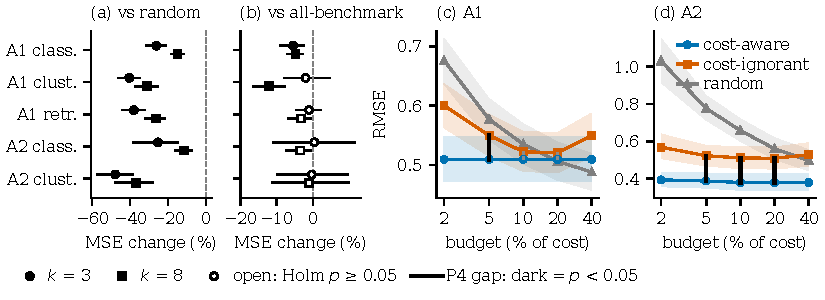
\includegraphics[width=\textwidth]{figures/f3.pdf}
\caption{Groups of tasks and unequal costs. (a, b) Group-targeted A-optimal selection minus random choice (a) and minus the all-benchmark complement-error greedy (b): relative change in group MSE (\%) at $k=3$ (circles) and $k=8$ (squares), 95\% intervals over held-out models; filled: Holm $p<0.05$ over the 20 declared tests. Class., clust., retr.: classification, clustering, retrieval tasks; A1, A2: MTEB-A1, MTEB-A2. (c, d) RMSE against the budget, the share of the summed median evaluation time of all benchmarks, for cost-aware and cost-ignorant A-optimal selection and random choice (bands: 95\%); segments join the two A-optimal choices (dark: Holm $p<0.05$ over six tests; grey dotted: not significant). Curves are evaluated on the $k$ grid; the cost-aware choice is the grid maximum for budgets above $1.7\%$ (A1) and $7\%$ (A2) of the total, so its curve is flat. Five repetitions.}
\label{fig:f3}
\end{figure}

\section{Inference rules at a fixed selection}
\label{app:rules}
\begin{figure}[h]
\centering
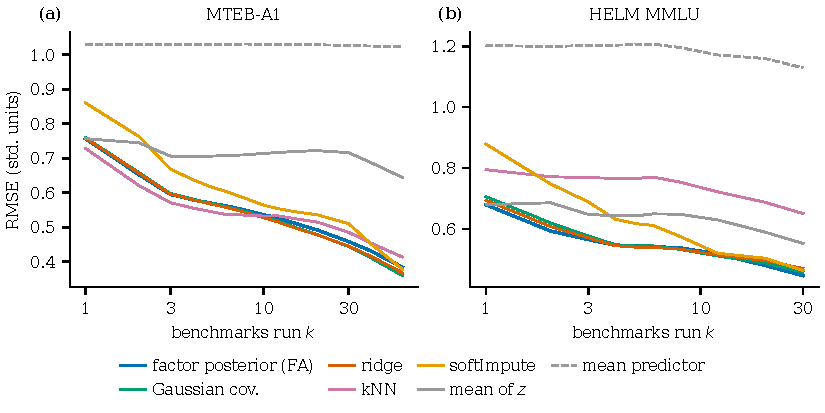
\includegraphics[width=\textwidth]{figures/f6_rules.pdf}
\caption{RMSE against $k$ for six inference rules and the history-mean predictor with the selection fixed (complement-error greedy$^\dagger$), on MTEB-A1 and HELM MMLU: factor posterior, Gaussian covariance conditioning with a shrunk covariance, ridge, kNN, softImpute and mean of the latent scores.}
\end{figure}

\section{Forecast against the size of the history}
\label{app:history}
Varying the history size $M$ (25 test models with their families excluded from the history, 10 repetitions) shows where this stops holding.
On MTEB the forecast is optimistic at every $M$ and the median absolute gap falls with $M$: on A1 $37$, $29$, $21$, $21$ and $18\%$ at $M=20$, $30$, $45$, $60$ and $78$ (within $20\%$ in $23\%$ of the $(M,k)$ cells), on A2 $79\%$ at $M=20$ and $17$--$22\%$ for $M\ge45$.
The selected rank is within 2 of the predicted one only when the history is nearly the whole matrix (A1: $0$, $0$, $10$, $40$ and $100\%$ of repetitions at the same $M$), whereas on the Open LLM Leaderboard matrices ($N=6$ and $40$, $M$ up to $2000$) the median gap is at most $1.2\%$ and $3.4\%$ at $M\ge500$ and the rank is within 2 in every repetition from $M=500$: the correction helps when $M$ is large against $N$ and under-resolves the rank when it is not.

\section{Unseen organisations and simple alternatives}
\label{app:fam}
The held-out models of a random fold share an organisation with models of the history, so the selection gain of Section~\ref{sec:experiments} may partly be an in-distribution effect.
We repeat the MTEB comparisons with the folds made of whole organisations (history without any test organisation) and resample organisations rather than models in the bootstrap; A1 and A2 use five repetitions, B three.
Table~\ref{tab:fam} gives the relative change in MSE of the comparisons of the primary family that involve random choice, and of two simple alternatives that we added after the pilot and did not include in the declared family: forward regression and $k$-medoids on the benchmark correlation.
Table~\ref{tab:famrmse} gives the RMSE.
The Holm correction is over the 15 tests of each matrix and regime and not over the family of Table~\ref{tab:t2}, so signs and significance, not $p$-values, are comparable.
\begin{table}[h]
\centering\scriptsize\setlength{\tabcolsep}{3pt}
\begin{tabular}{@{}ll@{\hspace{9pt}}rrr@{\hspace{9pt}}rrr@{\hspace{9pt}}rrr@{\hspace{9pt}}rrr@{}}
\toprule
& & \multicolumn{3}{c}{A-opt.} & \multicolumn{3}{c}{compl.\,$\dagger$} & \multicolumn{3}{c}{compl.\,$\dagger$} & \multicolumn{3}{c}{compl.\,$\dagger$} \\
& & \multicolumn{3}{c}{vs random} & \multicolumn{3}{c}{vs random} & \multicolumn{3}{c}{vs fwd. regr.} & \multicolumn{3}{c}{vs $k$-medoids} \\
\cmidrule(lr){3-5} \cmidrule(lr){6-8} \cmidrule(lr){9-11} \cmidrule(lr){12-14}
& & 3 & 8 & 20 & 3 & 8 & 20 & 3 & 8 & 20 & 3 & 8 & 20 \\
\midrule
A1 & random folds & \textbf{$-$28} & \textbf{$-$15} & \textbf{$-$3} & \textbf{$-$28} & \textbf{$-$15} & \textbf{$-$15} & $-$1 & $-$2 & \textbf{$-$6} & $+$3 & $-$2 & \textbf{$-$9} \\
 & held-out organisations & \textbf{$-$27} & \textbf{$-$11} & $-$2 & \textbf{$-$27} & \textbf{$-$12} & \textbf{$-$14} & $-$3 & $-$2 & $-$7 & 0 & $-$2 & \textbf{$-$9} \\
\addlinespace[2pt]
A2 & random folds & \textbf{$-$20} & $-$3 & \textbf{$+$52} & \textbf{$-$20} & \textbf{$-$32} & \textbf{$-$50} & $+$1 & \textbf{$-$5} & $-$4 & $+$2 & \textbf{$-$18} & \textbf{$-$37} \\
 & held-out organisations & $-$4 & $+$16 & \textbf{$+$62} & $-$4 & \textbf{$-$77} & \textbf{$-$85} & $-$1 & $-$79 & $-$4 & $+$3 & \textbf{$-$19} & \textbf{$-$38} \\
 & held-out, without one organisation$\,\ddagger$ & \textbf{$-$23} & 0 & \textbf{$+$49} & \textbf{$-$23} & \textbf{$-$24} & \textbf{$-$49} & $-$1 & $-$1 & $-$3 & $+$1 & \textbf{$-$12} & \textbf{$-$30} \\
\addlinespace[2pt]
B & random folds & \textbf{$-$22} & $-$2 & \textbf{$+$14} & \textbf{$-$22} & $-$3 & \textbf{$-$15} & \textbf{$-$9} & $+$7 & \textbf{$-$13} & $-$1 & \textbf{$+$5} & $-$16 \\
 & held-out organisations & \textbf{$-$13} & $+$1 & \textbf{$+$19} & \textbf{$-$12} & 0 & $+$8 & $-$1 & $+$2 & $-$2 & $+$2 & \textbf{$+$6} & $+$4 \\
\bottomrule
\end{tabular}

\caption{Relative change in held-out MSE (\%) at $k=3$, $8$, $20$, first named minus second (negative: first is better), by organisation bootstrap; \textbf{bold}: Holm-adjusted $p<0.05$ over 15 tests. compl.\,$\dagger$: complement-error greedy; each change is divided by the mean MSE of the second selector in the full sample, so an interval end below $-100\%$ is possible and is not an error reduced by more than all of it. The last two comparisons are exploratory. On A2 with held-out organisations the scale is an MSE dominated by one organisation, so the large magnitudes of that row ($-77$, $-79$) mark the tail rather than an effect. $^\ddagger$ The organisation \texttt{codefuse-ai} (8 models, 64\% of the mean-predictor MSE under held-out folds) removed after the fact. Intervals: \texttt{code/results/FAM/TABLES.md}.}
\label{tab:fam}
\end{table}
\begin{table}[h]
\centering\scriptsize\setlength{\tabcolsep}{3pt}
\begin{tabular}{@{}ll@{\hspace{9pt}}rrr@{\hspace{9pt}}rrr@{\hspace{9pt}}rrr@{}}
\toprule
& & \multicolumn{3}{c}{random} & \multicolumn{3}{c}{A-optimal} & \multicolumn{3}{c}{compl.\,$\dagger$} \\
\cmidrule(lr){3-5} \cmidrule(lr){6-8} \cmidrule(lr){9-11}
& & 3 & 8 & 20 & 3 & 8 & 20 & 3 & 8 & 20 \\
\midrule
A1 & random folds & 0.70 & 0.59 & 0.53 & 0.60 & 0.55 & 0.52 & 0.60 & 0.55 & 0.49 \\
 & held-out organisations & 0.74 & 0.64 & 0.59 & 0.63 & 0.60 & 0.58 & 0.63 & 0.60 & 0.54 \\
\addlinespace[2pt]
A2 & random folds & 0.63 & 0.52 & 0.47 & 0.56 & 0.51 & 0.58 & 0.56 & 0.43 & 0.33 \\
 & held-out organisations & 1.22 & 1.16 & 1.13 & 1.20 & 1.25 & 1.43 & 1.20 & 0.56 & 0.43 \\
 & held-out, without one organisation$\,\ddagger$ & 0.63 & 0.54 & 0.49 & 0.56 & 0.54 & 0.60 & 0.55 & 0.47 & 0.35 \\
\addlinespace[2pt]
B & random folds & 0.79 & 0.70 & 0.67 & 0.70 & 0.70 & 0.72 & 0.70 & 0.69 & 0.62 \\
 & held-out organisations & 1.08 & 1.00 & 0.96 & 1.01 & 1.00 & 1.05 & 1.01 & 1.00 & 1.00 \\
\bottomrule
\end{tabular}

\caption{RMSE in standardised units at $k=3$, $8$, $20$ with factor inference, random folds and folds of held-out organisations; compl.\,$\dagger$: complement-error greedy; $\ddagger$ as in Table~\ref{tab:fam}.}
\label{tab:famrmse}
\end{table}
For A1 the held-out organisations leave every direction unchanged; only the small gain of the A-optimal criterion at $k=20$ ($-3\%$ with random folds, $-2\%$ with held-out organisations) is no longer significant.
On A2 one organisation (\texttt{codefuse-ai}) carries 64\% of the mean-predictor error under held-out folds, and the RMSE over all held-out models exceeds 1 at $k=3$ for every selector; the A-optimal criterion is then no better than random choice at $k=3$ and $8$ and $62\%$ worse at $k=20$, whereas the complement-error greedy is better than random at $k=8$ and $20$, with intervals wide because of that tail.
Without that organisation the picture of random folds returns (the row marked $\ddagger$).
On B the gain of the complement-error greedy over random choice at $k=3$ holds ($-12\%$) and at $k=20$ it is a tie ($+8\%$, not significant) against $-15\%$ with random folds.
Resampling organisations widens the intervals of the paired differences by a median of $17\%$ (A1), $18\%$ (A2) and $38\%$ (B) and changes no decision of Table~\ref{tab:t2}.
Against the simple alternatives the complement-error greedy is never worse on A1 and A2 and better than $k$-medoids at $k=20$ ($-9\%$ and $-37\%$); on B it is worse than $k$-medoids at $k=8$ ($+5\%$ with random folds, $+6\%$ with held-out organisations, both significant) and not better than forward regression ($+7\%$, not significant).

\section{Shift}
\label{app:shift}
\begin{figure}[h]
\centering
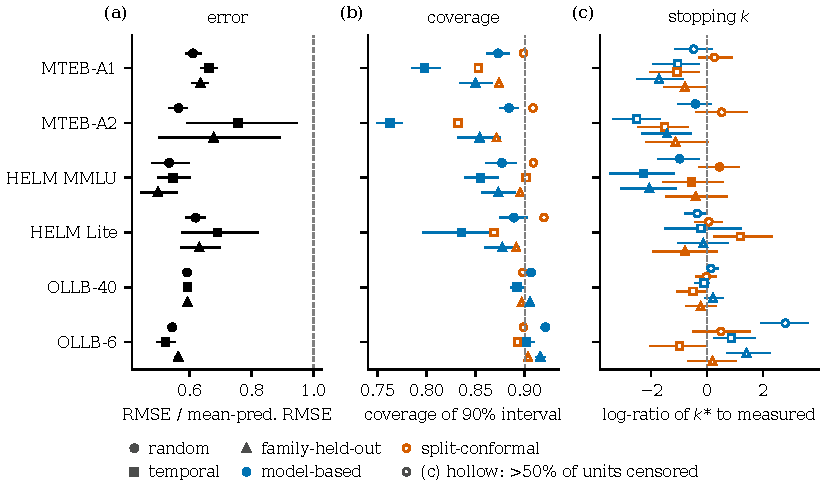
\includegraphics[width=\textwidth]{figures/f5.pdf}
\caption{Shift, A-optimal selection with factor inference, $k=3$ (the largest $k$ every matrix has). Markers: split. (a) RMSE over the mean-predictor RMSE. (b) Coverage of the nominal 90\% interval, model-based and split-conformal. (c) Error of the stopping $k$ (log$_2$ of the rule's $k^\ast$ over the measured $k^\ast$; tolerance 0.5); hollow markers: more than half of the units never reach the tolerance on the grid.}
\label{fig:f5}
\end{figure}
Under temporal splits the model-based intervals cover $0.76$ (A2) and $0.80$ (A1) of the scores at $k=3$, under family-held-out splits $0.85$, and on the generative-LLM matrices within $0.02$--$0.06$ of $0.90$ (panel b); split-conformal intervals cover $0.83$ and $0.85$ under temporal shift on MTEB.
The error relative to the mean predictor rises under temporal shift on MTEB and not on the Open LLM Leaderboard matrices (panel a).
The stopping $k$ of neither rule is uniformly closer to the measured one (panel c).

\section{Reproducing the results}
\label{app:repro}
All experiments run on CPU only.
The supplementary material contains the data extraction with the pinned versions of Appendix~\ref{app:data}, the analysis code (selectors, factor analysis with missing data, the protocol of Section~\ref{sec:setting}, the theory formulas), one driver script per experiment with its seeds, the result files from which every figure and table is drawn, and the scripts that draw them.
Jobs ran on two CPU cores each of a shared Intel Xeon Gold 6230 host, with 0.1--0.8 GB of memory, Python 3.11 with NumPy 2.4, SciPy 1.17, pandas 3.0 and scikit-learn 1.9, one BLAS thread per process; repetition $r$ seeds the split and every random draw with $r$.
Fitting the models of one repetition (five folds) takes a median of 3.5 minutes on A2 and 7.8 minutes on A1; the whole ten-repetition runs took about 33 minutes (A2) and 75 minutes (A1) of wall-clock time on the loaded host.
The leakage ablation takes 3 minutes (A1) and 1 minute (A2) per repetition, and the factor-model fits of the generative-LLM leaderboards 1 to 3 minutes per repetition, 26 and 36 minutes for the two Open LLM Leaderboard matrices.
The nonlinear imputers of Section~\ref{sec:experiments} dominate the cost on A1 (more than two hours for five repetitions on the full grid).
